\documentclass[11pt]{article}
\usepackage[margin=1in]{geometry}
\usepackage{graphicx}
\usepackage{booktabs}
\usepackage{float}
\usepackage{amsmath}
\usepackage{siunitx}
\usepackage[hidelinks]{hyperref}
\usepackage{caption}
\usepackage{array}
\usepackage{tabularx}
\usepackage{microtype}

\sisetup{
  round-mode=places,
  round-precision=3,
  group-separator={,},
}

\newcolumntype{Y}{>{\raggedright\arraybackslash}X}

\title{Pulse-Driven Magnetization Switching in a TDNEGF Spin-Electron Model:\\Self-Contained Physical Summary of Time-Domain Evidence, Controls, and Open Limits}
\author{Prepared from FermiLink/TDNEGF project artifacts}
\date{2026-04-16}

\begin{document}
\maketitle

\begin{abstract}
The central objective of this project is to determine whether an applied electrical pulse can drive a ferromagnetic nanostructure into a genuinely reversed magnetic state, and whether that statement survives the required control tests. The completed campaign now supports a qualified positive conclusion. A real switching regime exists, clean pulse-triggered reversal with retention is observed in a well-defined subset of parameter families, and matched pulse-minus-no-pulse subtraction reveals a pulse-specific nonequilibrium electronic signature that is absent before the drive and dominated by the component parallel to the switching axis. At the same time, the campaign also shows why switching claims cannot be based on final magnetization alone: pre-pulse drift can mimic success, delayed collapse can matter as much as the in-pulse minimum, and some families remain baseline-ambiguous even without the pulse. The strongest present statement is therefore selective rather than universal: pulse-driven switching is established for the clean Branch A and high-damping families, while the Branch B/\texttt{hsfull} neighborhood remains unresolved because the no-pulse baseline is itself near a sign-indefinite state.
\end{abstract}

\section{Physical objective and simulated system}
This report is written to be self-contained. The project studies a small ferromagnetic spin texture self-consistently coupled to itinerant electrons within a time-dependent nonequilibrium Green-function (TDNEGF) framework combined with classical spin dynamics. Operationally, the simulations use a \(2\times 2\) magnetic region (\(N_x=N_y=2\)) with one orbital per site (\(N_{\mathrm{orb}}=1\)), two spin projections (\(N_\sigma=2\)), and two electronic leads (\(N_\alpha=2\)). The initial magnetic configuration is ferromagnetic (FM), and the system is driven by a right-lead pulse while the left lead remains unbiased.

The main project-level question is:
\begin{quote}
Can the pulse produce \emph{physical magnetization switching}, meaning a reversal that is time-locked to the drive, survives after the drive, and cannot be explained by the corresponding no-pulse evolution?
\end{quote}

The magnetic observable used throughout is the spatially averaged \(z\)-component of the local moments,
\[
\langle M_z\rangle(t)=\frac{1}{N}\sum_i M_{i,z}(t),
\]
where \(+z\) is the initial easy-axis direction and \(-z\) is the reversed state. The electronic observable used to diagnose the driving mechanism is the excess spin density
\[
\sigma_{\Delta,\alpha i}(t)=\sigma_{\alpha i}(t)-\sigma^{\mathrm{eq}}_{\alpha i},
\]
resolved by Cartesian component \(\alpha\in\{x,y,z\}\) and site \(i\).

\section{Simulation protocol, nomenclature, and explicit parameters}
Two points need to be stated explicitly because the previous manuscript assumed too much prior context.

First, the labels \textbf{Branch A}, \textbf{Branch B}, and \textbf{Branch C} are campaign-internal names for distinct parameter families used in the focused follow-up scan. They are \emph{not} magnon branches or analytic branches of the equations of motion.

Second, the suffixes \texttt{hsneq} and \texttt{hsfull} are not cosmetic names. They correspond to the simulation flag \texttt{Hs\_update\_mode}:
\begin{itemize}
\item \texttt{hsneq} \(=\) \texttt{nonequilibrium\_only}: the backaction update uses the nonequilibrium spin-density contribution only;
\item \texttt{hsfull} \(=\) \texttt{full\_spin\_density}: the update uses the full spin density.
\end{itemize}

Table~\ref{tab:common-params} lists the parameters that remain fixed across the focused switching campaign. Table~\ref{tab:family-params} then gives the explicit parameter values for the families discussed in this report.

\begin{table}[H]
\centering
\caption{Common simulation settings used in the focused switching study.}
\label{tab:common-params}
\small
\begin{tabularx}{\textwidth}{>{\raggedright\arraybackslash}p{0.26\textwidth} >{\raggedright\arraybackslash}p{0.15\textwidth} Y}
\toprule
Quantity & Value & Meaning \\
\midrule
Magnetic region size & \(N_x=N_y=2\) & Four local moments in a \(2\times 2\) ferromagnetic cluster \\
Spin/electronic channels & \(N_\sigma=2\), \(N_{\mathrm{orb}}=1\), \(N_\alpha=2\) & Two spin projections, one orbital per site, and two leads \\
Initial state & FM & Uniform positive-\(z\) ferromagnetic initial condition \\
Time step & \(dt=0.1\) & Integration sampling interval \\
Start/end times & \(t_0=0\), \(t_{\mathrm{end}}=5000\) or \(6000\) & \(t_{\mathrm{end}}=6000\) for pulse width \(3000\); otherwise \(5000\) \\
Pulse timing & \(t_{\mathrm{start}}=1000\), ramp \(=5\) & Pulse turns on after a long pre-pulse baseline \\
Lead bias convention & left scale \(=0\), right scale \(=1\) & Right-lead-only pulse drive \\
Magnetic field & \(B_x=0\) & No transverse static field used in these runs \\
Temperature parameters & \(\beta=33\), \(kT=0\) & Low-temperature / effectively zero-temperature working point in the saved parameter files \\
Lead coupling / lattice scale & \(\gamma=1.0\), \(a_0=1.0\) & Electronic coupling and lattice-unit conventions from the run inputs \\
Equilibrium contour settings & \(N_{\lambda 1}=49\), \(N_{\lambda 2}=20\) & Numerical TDNEGF contour settings used in the production runs \\
Solver tolerances & \texttt{reltol}\(=10^{-6}\), \texttt{abstol}\(=10^{-8}\) & ODE/integration tolerances from the saved input files \\
\bottomrule
\end{tabularx}
\normalsize
\end{table}

\begin{table}[H]
\centering
\caption{Explicit parameter values for the parameter families discussed in the report. The Branch names are campaign labels rather than physical branches.}
\label{tab:family-params}
\small
\begin{tabularx}{\textwidth}{>{\raggedright\arraybackslash}p{0.19\textwidth} >{\raggedright\arraybackslash}p{0.15\textwidth} >{\raggedright\arraybackslash}p{0.07\textwidth} >{\raggedright\arraybackslash}p{0.07\textwidth} >{\raggedright\arraybackslash}p{0.07\textwidth} >{\raggedright\arraybackslash}p{0.07\textwidth} >{\raggedright\arraybackslash}p{0.08\textwidth} >{\raggedright\arraybackslash}p{0.09\textwidth} Y}
\toprule
Family label & \texttt{Hs\_update\_mode} & pulse amp. & \(\gamma_{\mathrm{so}}\) & \(j_{sd}\) & \(j_{ex}\) & \(j_{ani}\) & damping & Pulse width(s) and role \\
\midrule
Branch A main & \texttt{nonequilibrium\_only} & 1.5 & 0.9 & 0.3 & -0.02 & 0.01 or 0.03 & 0.3 or 0.7 & widths \(1000, 2000, 3000\); clean switching-prone family \\
Branch A high damping strip & \texttt{nonequilibrium\_only} & 1.5 & 0.9 & 0.3 & -0.02 & 0.03 & 1.0 & width \(1000\); clean high-damping retention strip \\
Branch B main & \texttt{full\_spin\_density} & 2.0 or 2.25 & 0.9 & 0.3 & -0.01 & 0.0 & 0.4--0.7 & widths \(2500, 3000\); attractive pulsed traces but ambiguous no-pulse baseline \\
Branch C crosscheck & paired \texttt{hsneq}/\texttt{hsfull} & 1.5 or 2.0 & 0.9 & 0.3 & -0.02 or -0.01 & 0.03 or 0.0 & 0.3 or 0.5 & narrow paired comparison strip used only for mode cross-checks \\
\bottomrule
\end{tabularx}
\normalsize
\end{table}

For the earlier broad scan that first mapped the switching-prone regime, the explicit explored values were:
\[
\text{pulse amp.}\in\{1.5,2.0\},\quad
\gamma_{\mathrm{so}}\in\{0.7,0.9\},\quad
j_{sd}\in\{0.2,0.3\},
\]
\[
j_{ex}\in\{-0.02,-0.01\},\quad
j_{ani}\in\{0.0,0.03,0.05,0.08,0.10\},\quad
\text{damping}\in\{0.3,0.5\},
\]
with fixed pulse width \(1500\), pulse start \(1000\), and both \texttt{hsneq} and \texttt{hsfull} tested at each parameter point.

\section{Decision criteria for calling something switching}
The project uses three time-domain criteria to decide whether a trajectory is physically defensible as pulse-driven switching:
\begin{enumerate}
\item \textbf{clean pre-pulse behavior}: the run remains in the initial positive basin before pulse onset;
\item \textbf{pulse-locked response}: the dominant drop or sign crossing occurs during or after the pulse, not long before it;
\item \textbf{retention}: the reversed state persists after the pulse rather than rebounding back toward \(+z\).
\end{enumerate}

The same logic is applied to the electronic observables. A large raw \(\sigma_\Delta\) signal alone is not sufficient because startup transients can appear in both pulsed and unpulsed runs. The physically informative quantity is the matched subtraction
\[
\Delta \sigma_{\alpha,i}(t)=
\sigma^{\mathrm{pulse}}_{\alpha,i}(t)-\sigma^{\mathrm{no\ pulse}}_{\alpha,i}(t),
\]
which removes the shared baseline and isolates the pulse-specific excess.

\section{Campaign picture in one compact summary}
Table~\ref{tab:picture} condenses how each completed dataset contributes to the project-level switching claim.

\begin{table}[H]
\centering
\caption{Role of each dataset in the final physical interpretation.}
\label{tab:picture}
\small
\begin{tabularx}{\textwidth}{>{\raggedright\arraybackslash}p{0.21\textwidth} >{\raggedright\arraybackslash}p{0.26\textwidth} Y}
\toprule
Dataset layer & Physical question & Main conclusion \\
\midrule
Broad scan (\(320\) branch runs) & Does any robust switching-prone region exist at all? & Yes. Large pulse-window drops are real, especially at low anisotropy, but final-state ranking alone strongly overcounts physically valid switching because some runs drift negative before the pulse. \\
Focused follow-up (\(117\) runs) & Can selected candidates become retained reversed states? & Yes. Clean retained switching is reproducible in Branch A and in the high-damping strip. Two routes appear: strong in-pulse inversion and delayed post-pulse collapse. \\
No-pulse controls & Would the same family reverse without the pulse? & For the clean Branch A families, no. For Branch B/\texttt{hsfull}, the baseline itself is too close to reversal, so that family remains unresolved. \\
Pulse-minus-no-pulse subtraction & Is there a pulse-specific electronic signature beyond startup transients? & Yes in the clean families. The excess is zero before the pulse, turns on only after onset, and is consistently dominated by the \(z\) component. \\
Long-time no-pulse relaxation checks & Is the baseline electronic excess a persistent artifact? & The no-pulse excess decays strongly with time, supporting the use of matched subtraction rather than raw \(\sigma_\Delta\) amplitudes. \\
\bottomrule
\end{tabularx}
\normalsize
\end{table}

\section{Where the switching-prone regime first appears}
The broad scan established an important negative result before it established a positive one: a negative final \(\langle M_z\rangle\) is not, by itself, evidence of pulse-driven switching.

Across the completed broad scan:
\begin{itemize}
\item \(320\) branch runs were analyzed;
\item \(45\) changed final sign;
\item only \(1\) reached a strong final reversed state with \(\langle M_z\rangle_{\mathrm{final}}\le -0.8\);
\item that formally strongest final case had already crossed both \(0\) and \(-0.8\) \emph{before} pulse onset and therefore fails the clean switching criterion.
\end{itemize}

Once the time-domain gate is imposed, the physics becomes clearer:
\begin{itemize}
\item \(95\) runs show a large clean pulse-window drop;
\item \(94\) show a clean pulse-window crossing of \(\langle M_z\rangle=0\);
\item only \(1\) shows a clean pulse-window crossing of \(\langle M_z\rangle=-0.8\).
\end{itemize}

The strong message is that the drive can clearly destabilize the initial state, but true retained reversal is much rarer than raw sign changes suggest. The broad scan also identifies the main control parameter trend: low anisotropy is the gateway into strong response, whereas \(j_{ani}\ge 0.08\) does not even produce final sign changes in the tested grid.

\begin{figure}[H]
  \centering
  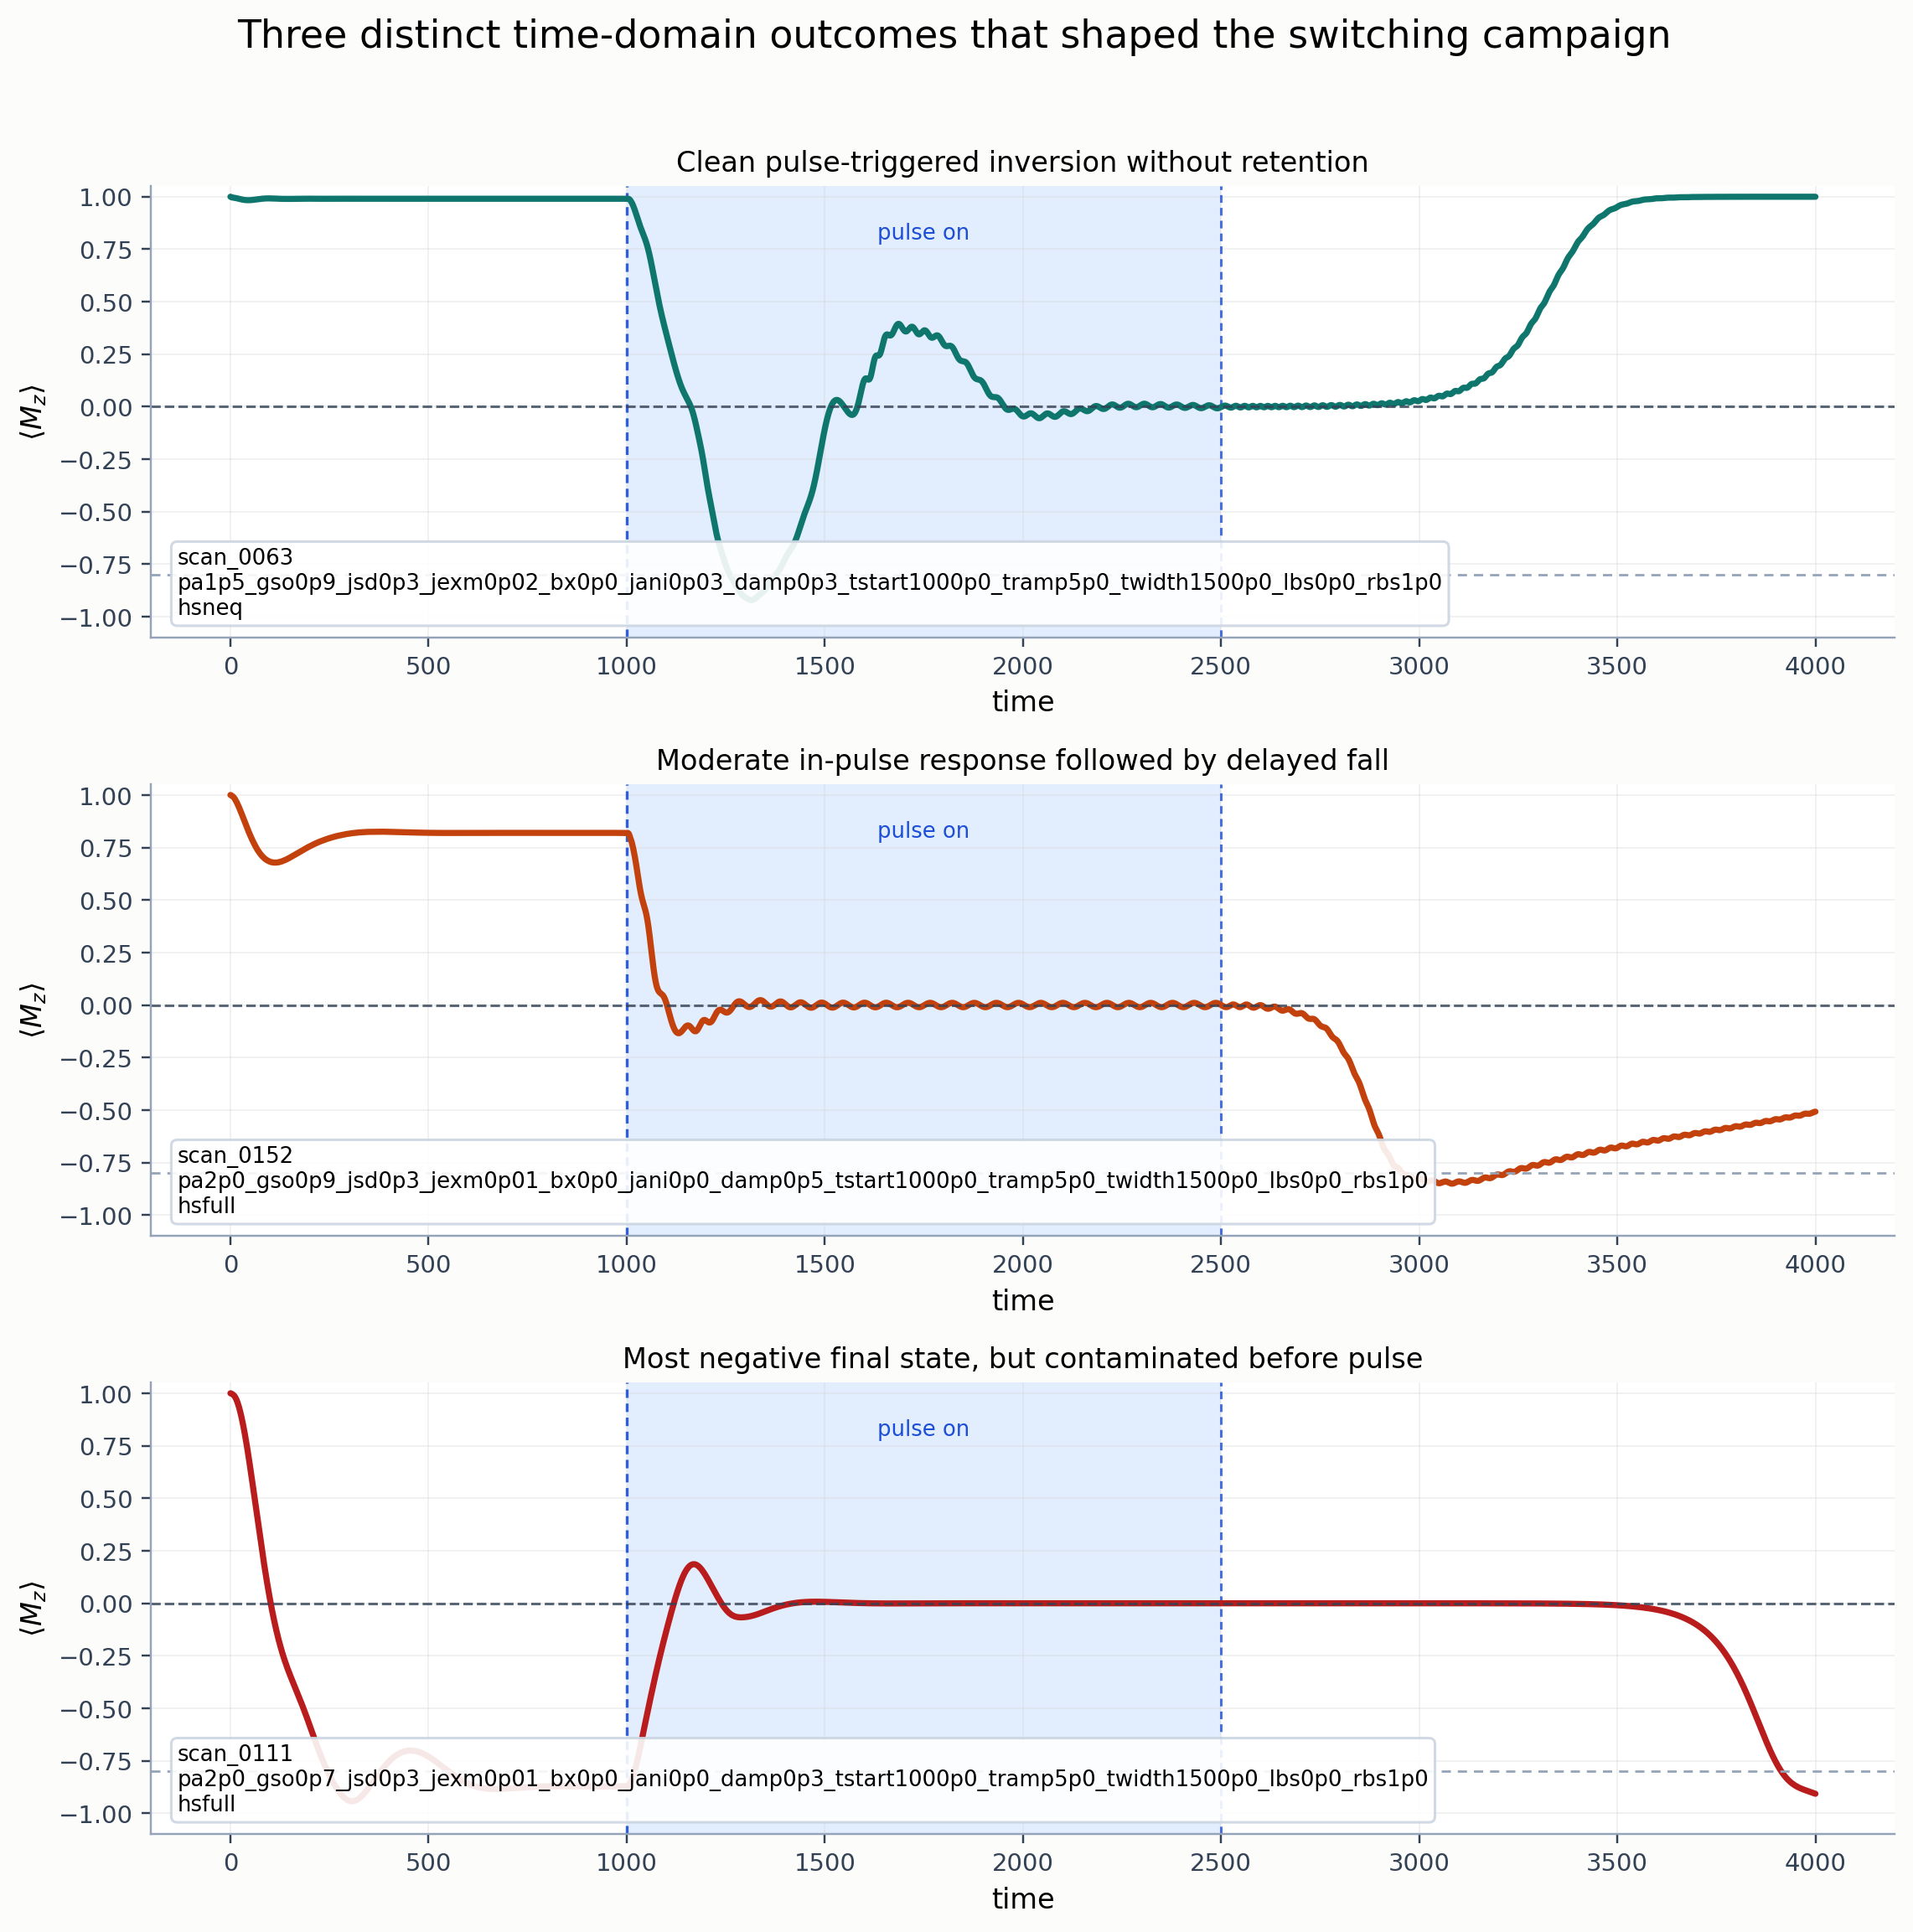
\includegraphics[width=0.9\textwidth]{figures/goal5_representative_dynamics.png}
  \caption{Representative time traces from the broad scan. The first panel shows a clean pulse-triggered inversion that later rebounds. The second shows a more moderate in-pulse response followed by a later fall. The third is the formally strongest negative final state in the scan, but it is not admissible as evidence for pulse-driven switching because it is already negative before the pulse begins.}
  \label{fig:goal5-dynamics}
\end{figure}

\section{How clean retained switching appears in time}
The focused follow-up was designed to test whether the switching-prone region can be converted into stable retained reversal. The answer is yes, but only for a subset of families.

Among the \(117\) completed focused runs:
\begin{itemize}
\item \(6\) reach strong in-pulse inversion, defined by \(\langle M_z\rangle\le -0.8\) during the pulse window;
\item \(20\) reach strong retained reversal at the final time;
\item the cleanest direct-switch case is \texttt{goal6\_A\_main\_0003}, with pulse minimum \(-0.9205\) and final \(-0.9997\);
\item the clearest delayed-retention case is \texttt{goal6\_A\_main\_0034}, with pulse minimum only \(-0.1166\) but final \(-0.9999\).
\end{itemize}

This distinction matters physically. The campaign does not show a single universal switching waveform. Instead, it shows at least two successful dynamical pathways:
\begin{enumerate}
\item a strong pulse-synchronous inversion that remains in the reversed basin;
\item a weaker or incomplete in-pulse response that seeds a continued post-pulse collapse toward \(-z\).
\end{enumerate}

\begin{figure}[H]
  \centering
  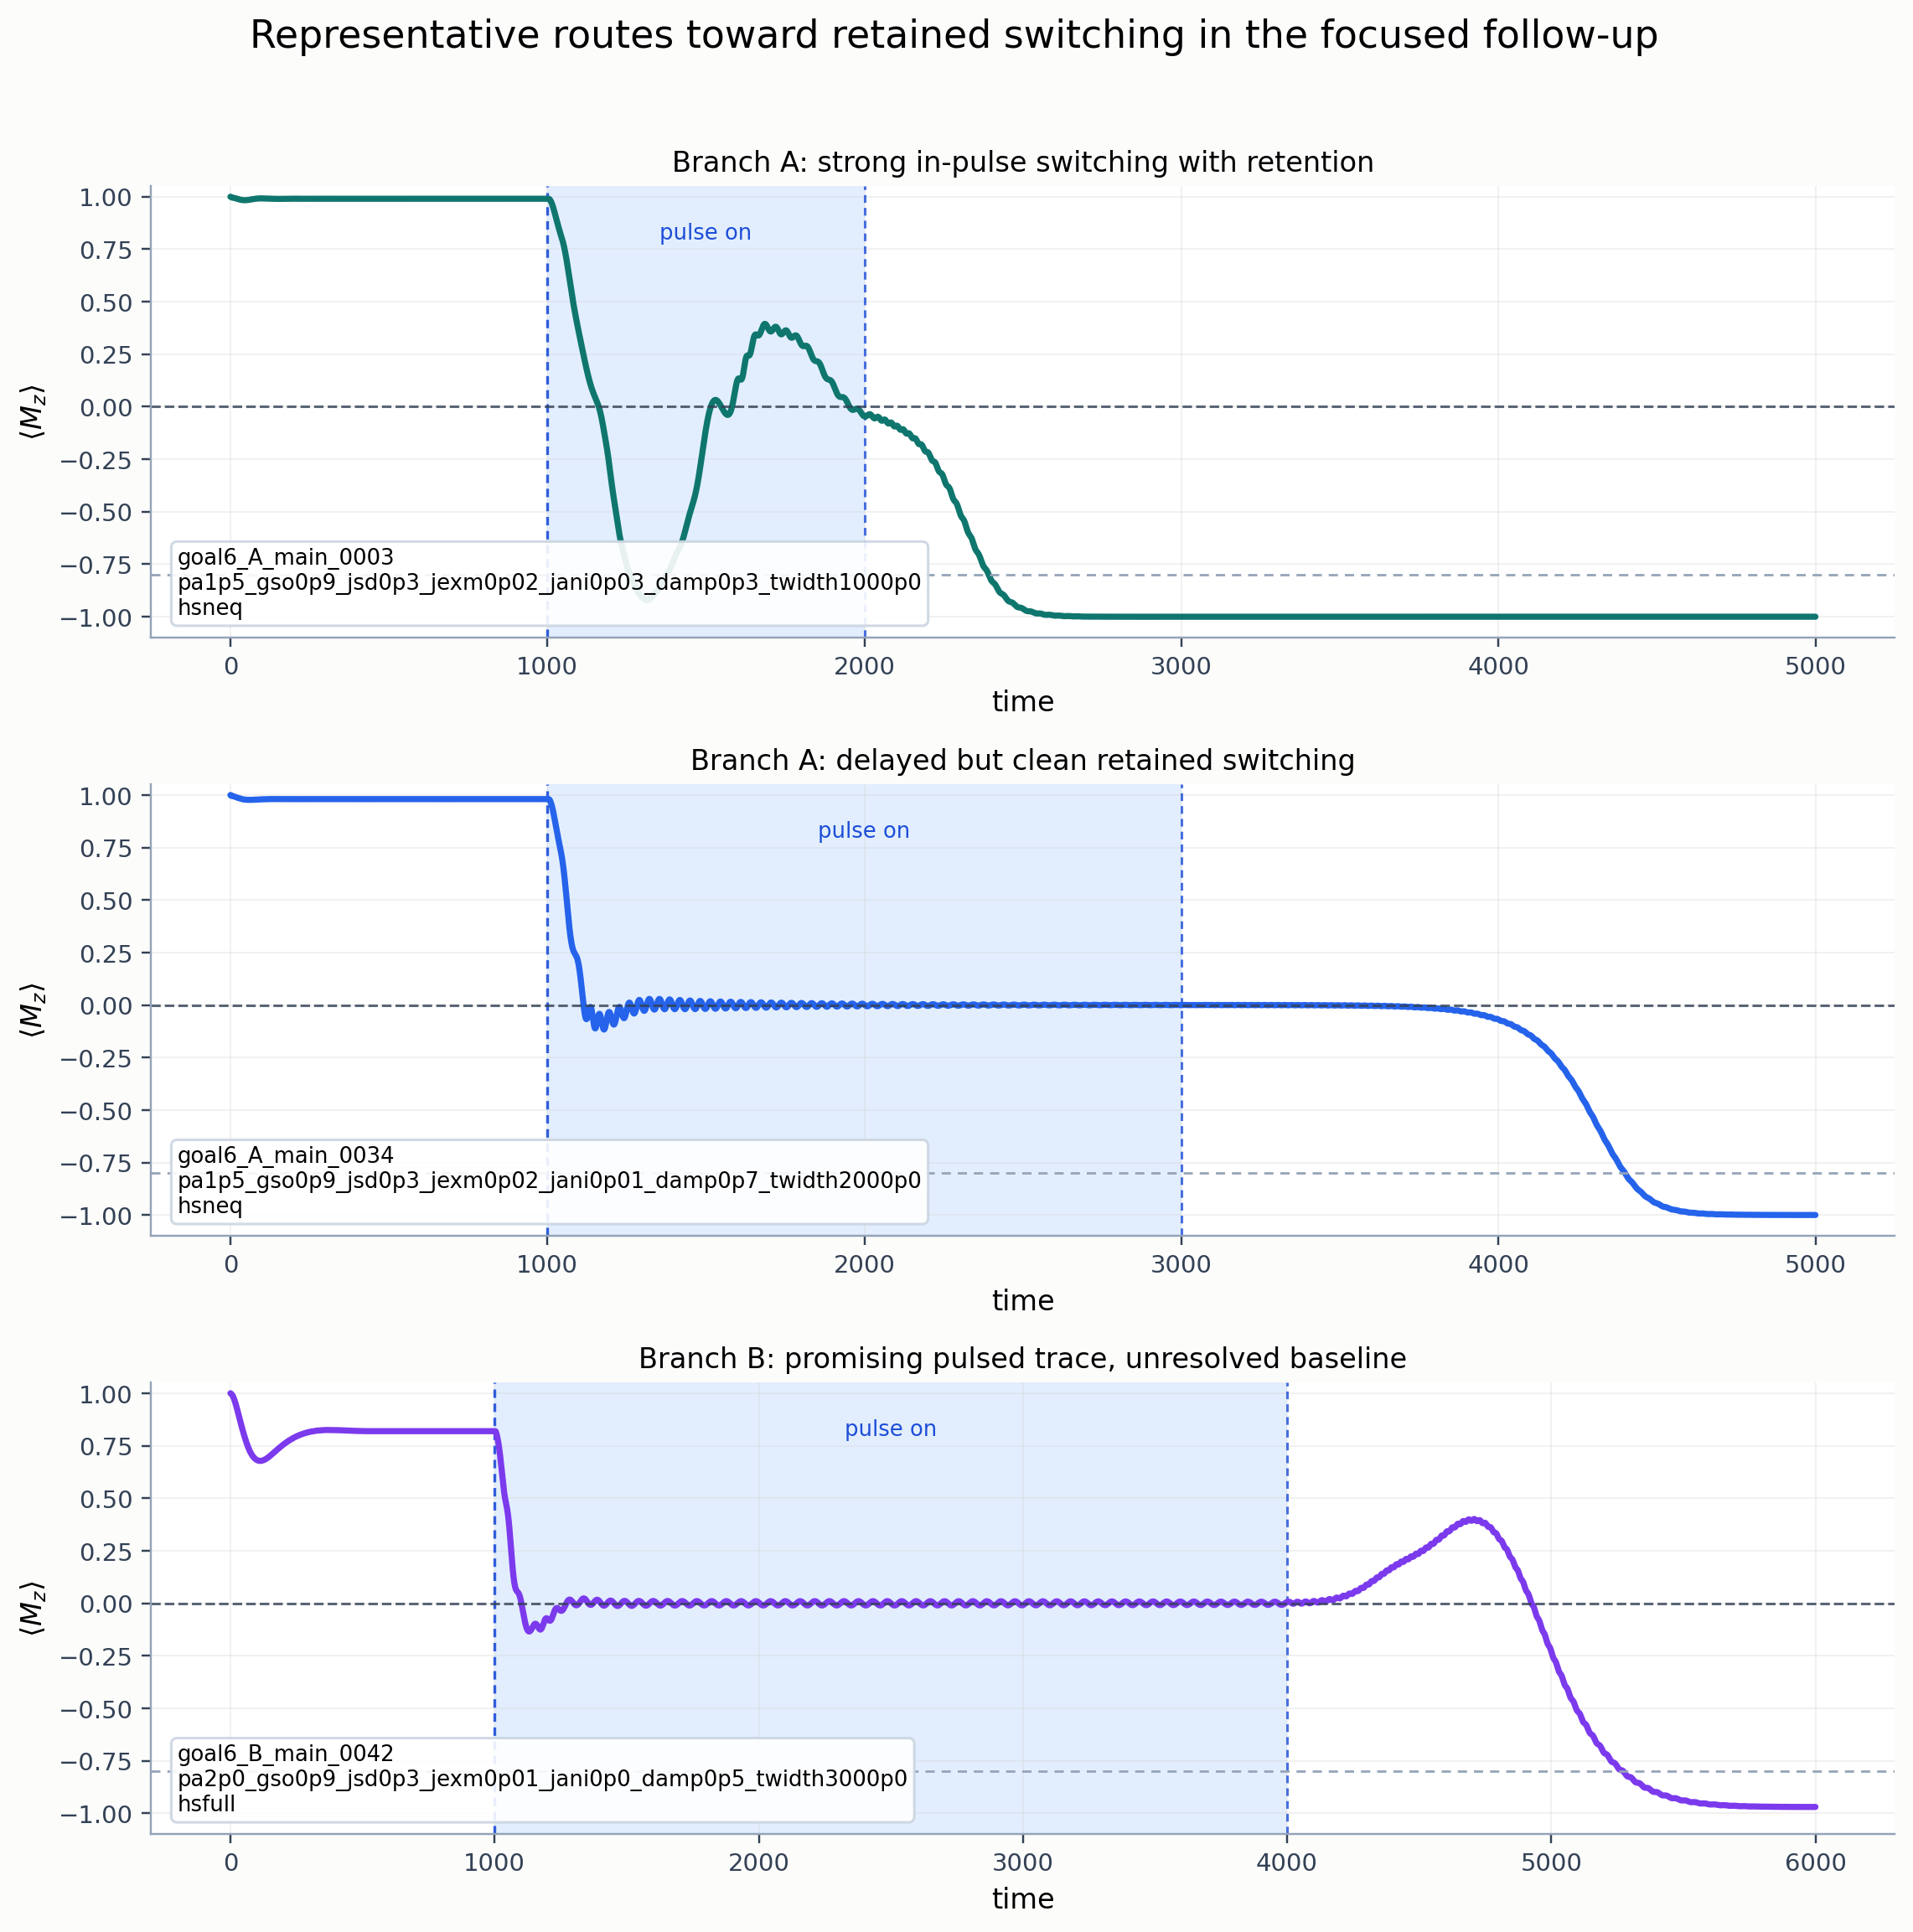
\includegraphics[width=0.9\textwidth]{figures/goal6_representative_dynamics.png}
  \caption{Representative retained-switching trajectories from the focused follow-up. The first two traces are clean Branch A cases and demonstrate the two successful pathways: prompt in-pulse switching and delayed post-pulse collapse. The third Branch B trace looks promising in isolation, but later no-pulse controls show that its local baseline is ambiguous.}
  \label{fig:goal6-dynamics}
\end{figure}

\section{Why the no-pulse controls are physically decisive}
No-pulse controls are not bookkeeping. They answer the core causality question: would the family reverse, or nearly reverse, even without the applied pulse?

The first result is favorable. In the no-pulse relaxation diagnostics, the electronic excess does not stay indefinitely at the pulse-scale amplitude. Instead it decays substantially with time. In the long-time check shown in Fig.~\ref{fig:rhoeq-relax}, the late-time envelope reaches approximately
\[
\max_{i,\alpha}|\sigma_{\Delta,\alpha i}(t)|\approx 8.9\times 10^{-3}
\quad \text{by } t=2000.
\]
That supports the interpretation that startup electronics generate a decaying background rather than a self-sustained pulse-like signal.

\begin{figure}[H]
  \centering
  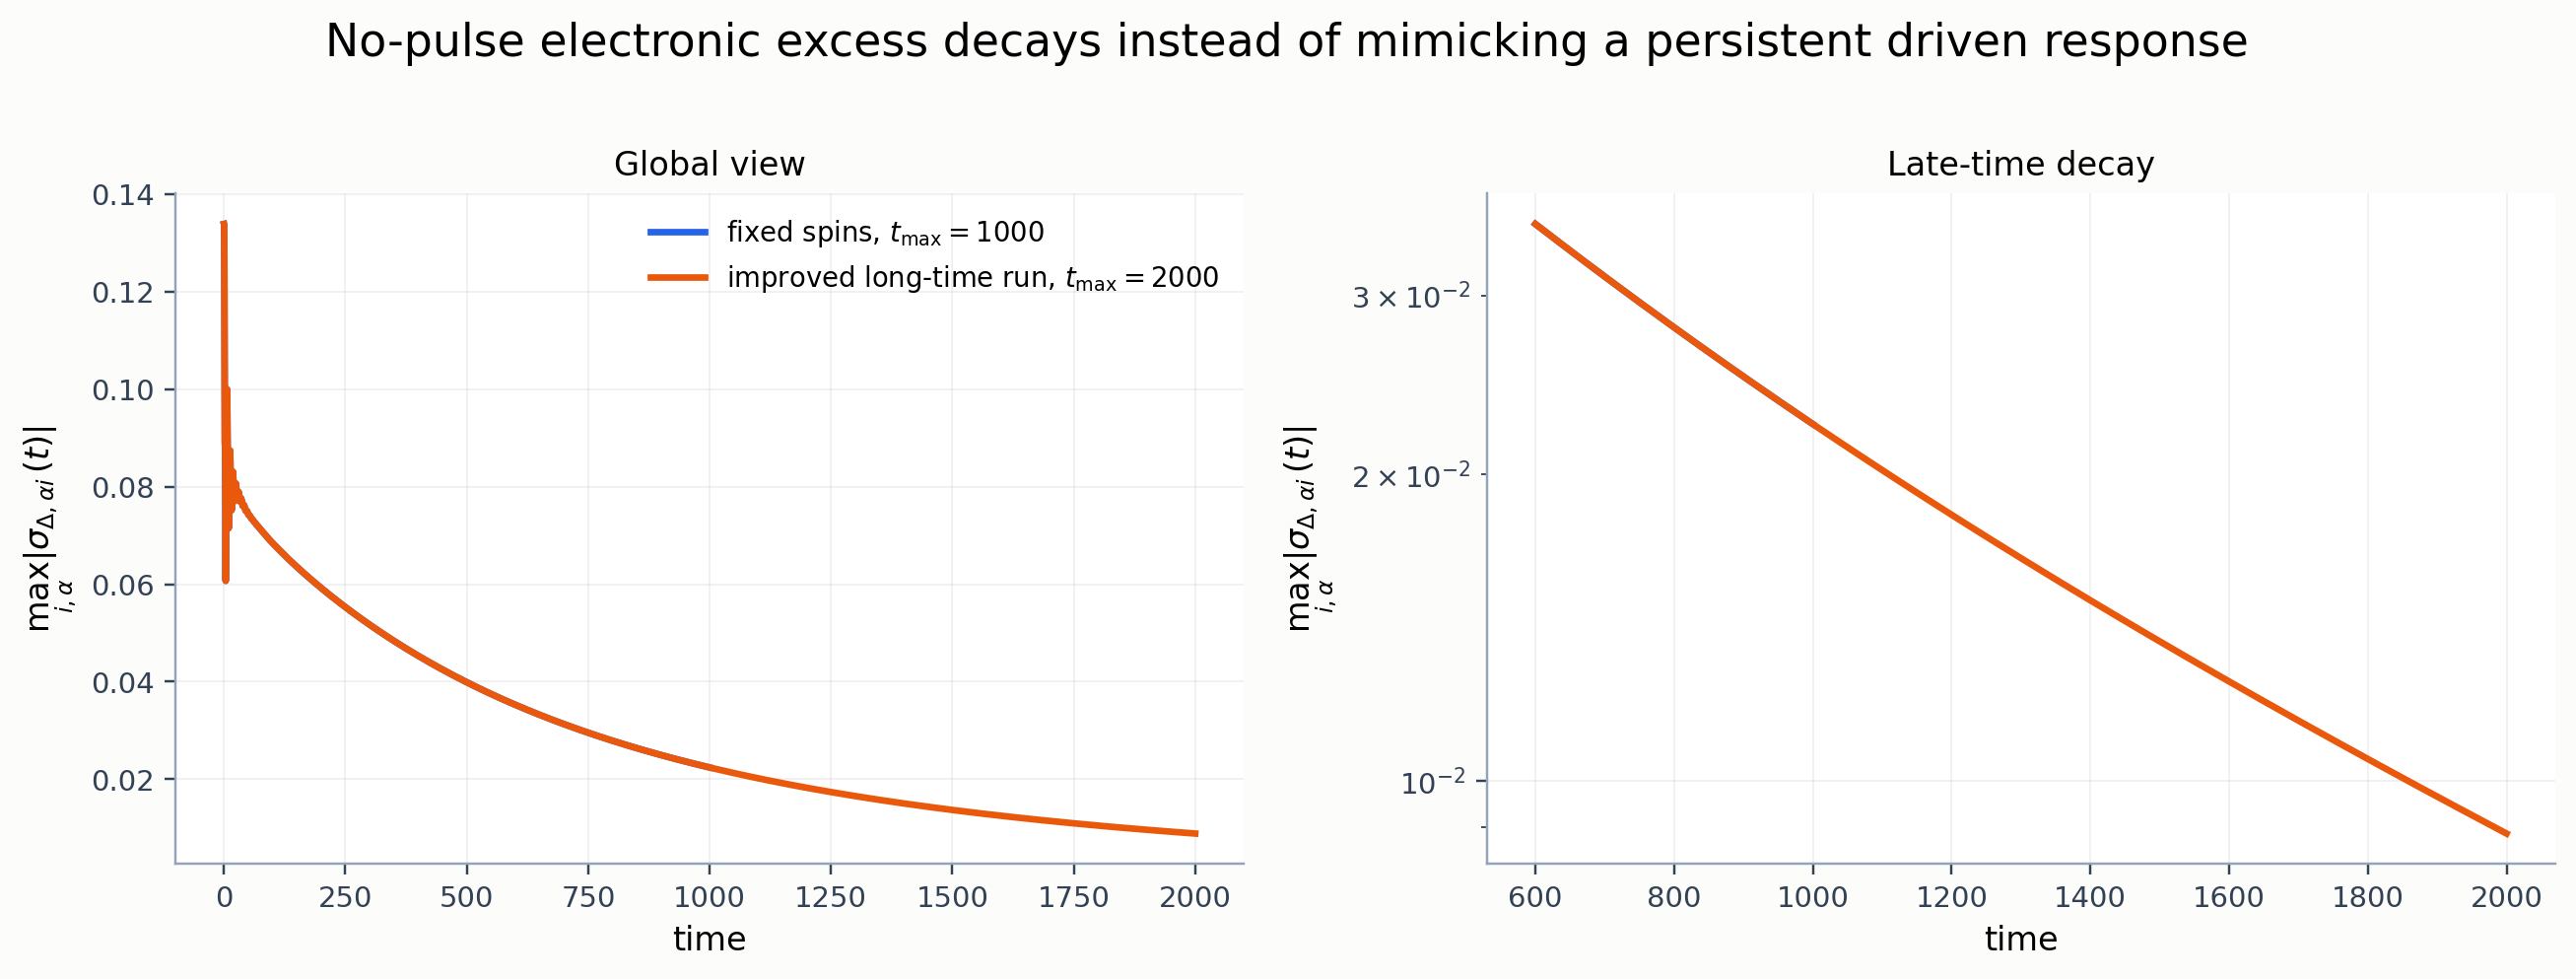
\includegraphics[width=0.92\textwidth]{figures/rhoeq_relaxation_tendency.png}
  \caption{No-pulse relaxation diagnostics for the electronic excess. The excess decays strongly in time rather than remaining at the scale associated with the switching-relevant pulse response. This is why the report interprets matched pulse-minus-no-pulse subtraction, not raw \(\sigma_\Delta\), as the decisive electronic observable.}
  \label{fig:rhoeq-relax}
\end{figure}

The second result is a warning. In Branch B/\texttt{hsfull}, the no-pulse baseline is itself close to reversal. Table~\ref{tab:branchb-controls} shows the family-neighbor follow-up around the ambiguous reference case \texttt{goal6\_B\_main\_0042}. Every tested no-pulse neighbor develops a negative excursion, and one remains slightly negative at the final time. That means the local baseline is already sign-indefinite in the absence of the drive.

\begin{table}[H]
\centering
\caption{Branch B/\texttt{hsfull} no-pulse follow-up. These controls block a universal switching claim because the family is already close to reversal without the pulse.}
\label{tab:branchb-controls}
\small
\begin{tabularx}{\textwidth}{>{\raggedright\arraybackslash}p{0.18\textwidth} >{\raggedright\arraybackslash}p{0.08\textwidth} >{\raggedright\arraybackslash}p{0.08\textwidth} >{\raggedright\arraybackslash}p{0.08\textwidth} >{\raggedright\arraybackslash}p{0.09\textwidth} >{\raggedright\arraybackslash}p{0.11\textwidth} Y}
\toprule
Case & pulse amp. & damping & width & \(\langle M_z\rangle_{\mathrm{min}}\) & \(\langle M_z\rangle_{\mathrm{final}}\) & Interpretation \\
\midrule
\texttt{0030} & 2.0 & 0.5 & 2500 & -0.1527 & 0.0156 & Crosses negative even without the pulse \\
\texttt{0035} & 2.25 & 0.7 & 2500 & -0.0536 & 0.0016 & Ends nearly zero after a negative excursion \\
\texttt{0041} & 2.0 & 0.4 & 3000 & -0.2322 & -0.0066 & Slightly negative final state without the pulse \\
\texttt{0043} & 2.0 & 0.7 & 3000 & -0.0536 & 0.0000 & Returns near zero, but only after crossing negative \\
\bottomrule
\end{tabularx}
\normalsize
\end{table}

\begin{figure}[H]
  \centering
  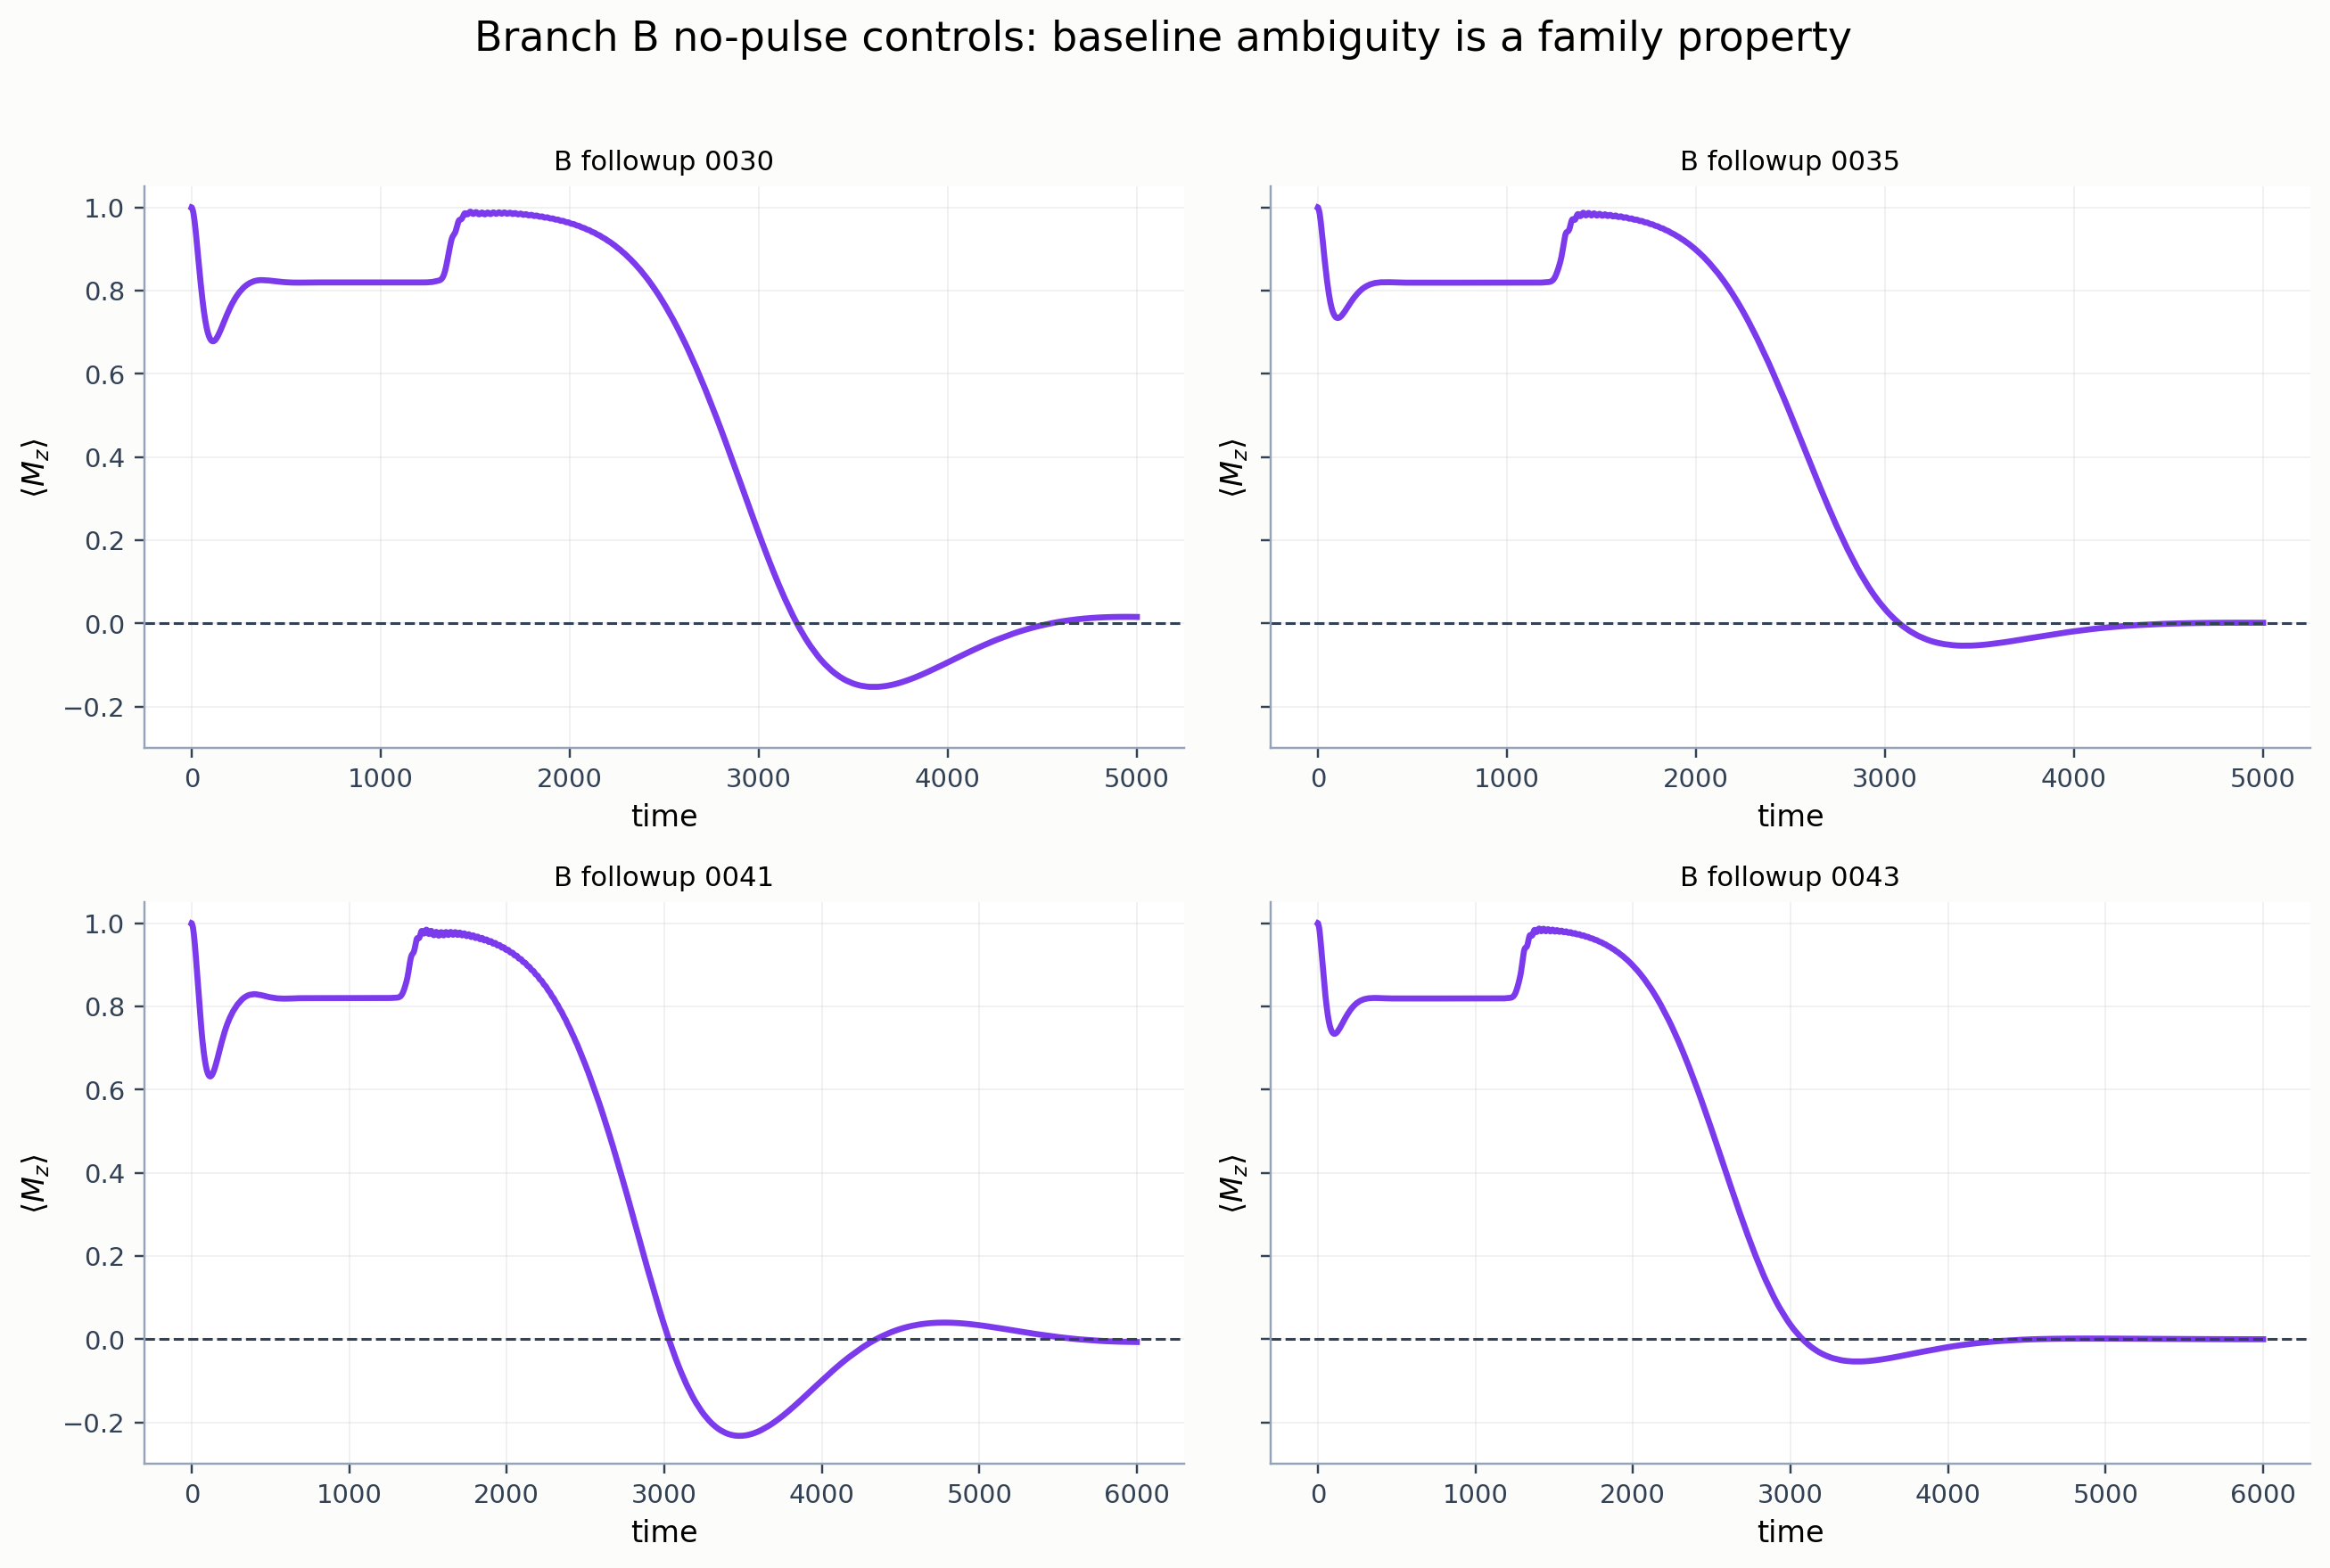
\includegraphics[width=0.95\textwidth]{figures/branchb_nopulse_followup_avgMz_grid.png}
  \caption{No-pulse trajectories in the Branch B/\texttt{hsfull} neighborhood. The family-level behavior is baseline-ambiguous: all cases show negative excursions and one ends slightly negative. This is why Branch B is labeled unresolved rather than successful or failed.}
  \label{fig:branchb-followup}
\end{figure}

\section{Mechanistic evidence from matched pulse-minus-no-pulse subtraction}
Once the ambiguous families are removed, the project reaches its strongest mechanistic result. Five matched pulse/control pairs satisfy the clean-family criteria. In every one of them:
\begin{itemize}
\item the pulsed run finishes near \(\langle M_z\rangle\approx -1\);
\item the matched no-pulse control remains near \(\langle M_z\rangle\approx +1\);
\item the pulse-minus-no-pulse electronic excess is exactly zero before pulse onset in the saved analysis table;
\item the dominant excess component is always \(z\), which is the axis of reversal.
\end{itemize}

The direct magnetic comparison is shown in Fig.~\ref{fig:clean-avgmz}. The pulse and control members begin from the same positive basin, but only the driven member crosses into the reversed state and stays there. The corresponding matched electronic subtraction in Fig.~\ref{fig:clean-excess} is even more constraining: the excess is absent before the pulse, turns on only after \(t_{\mathrm{start}}=1000\), and is largest in the \(z\) component for every clean pair.

\begin{figure}[H]
  \centering
  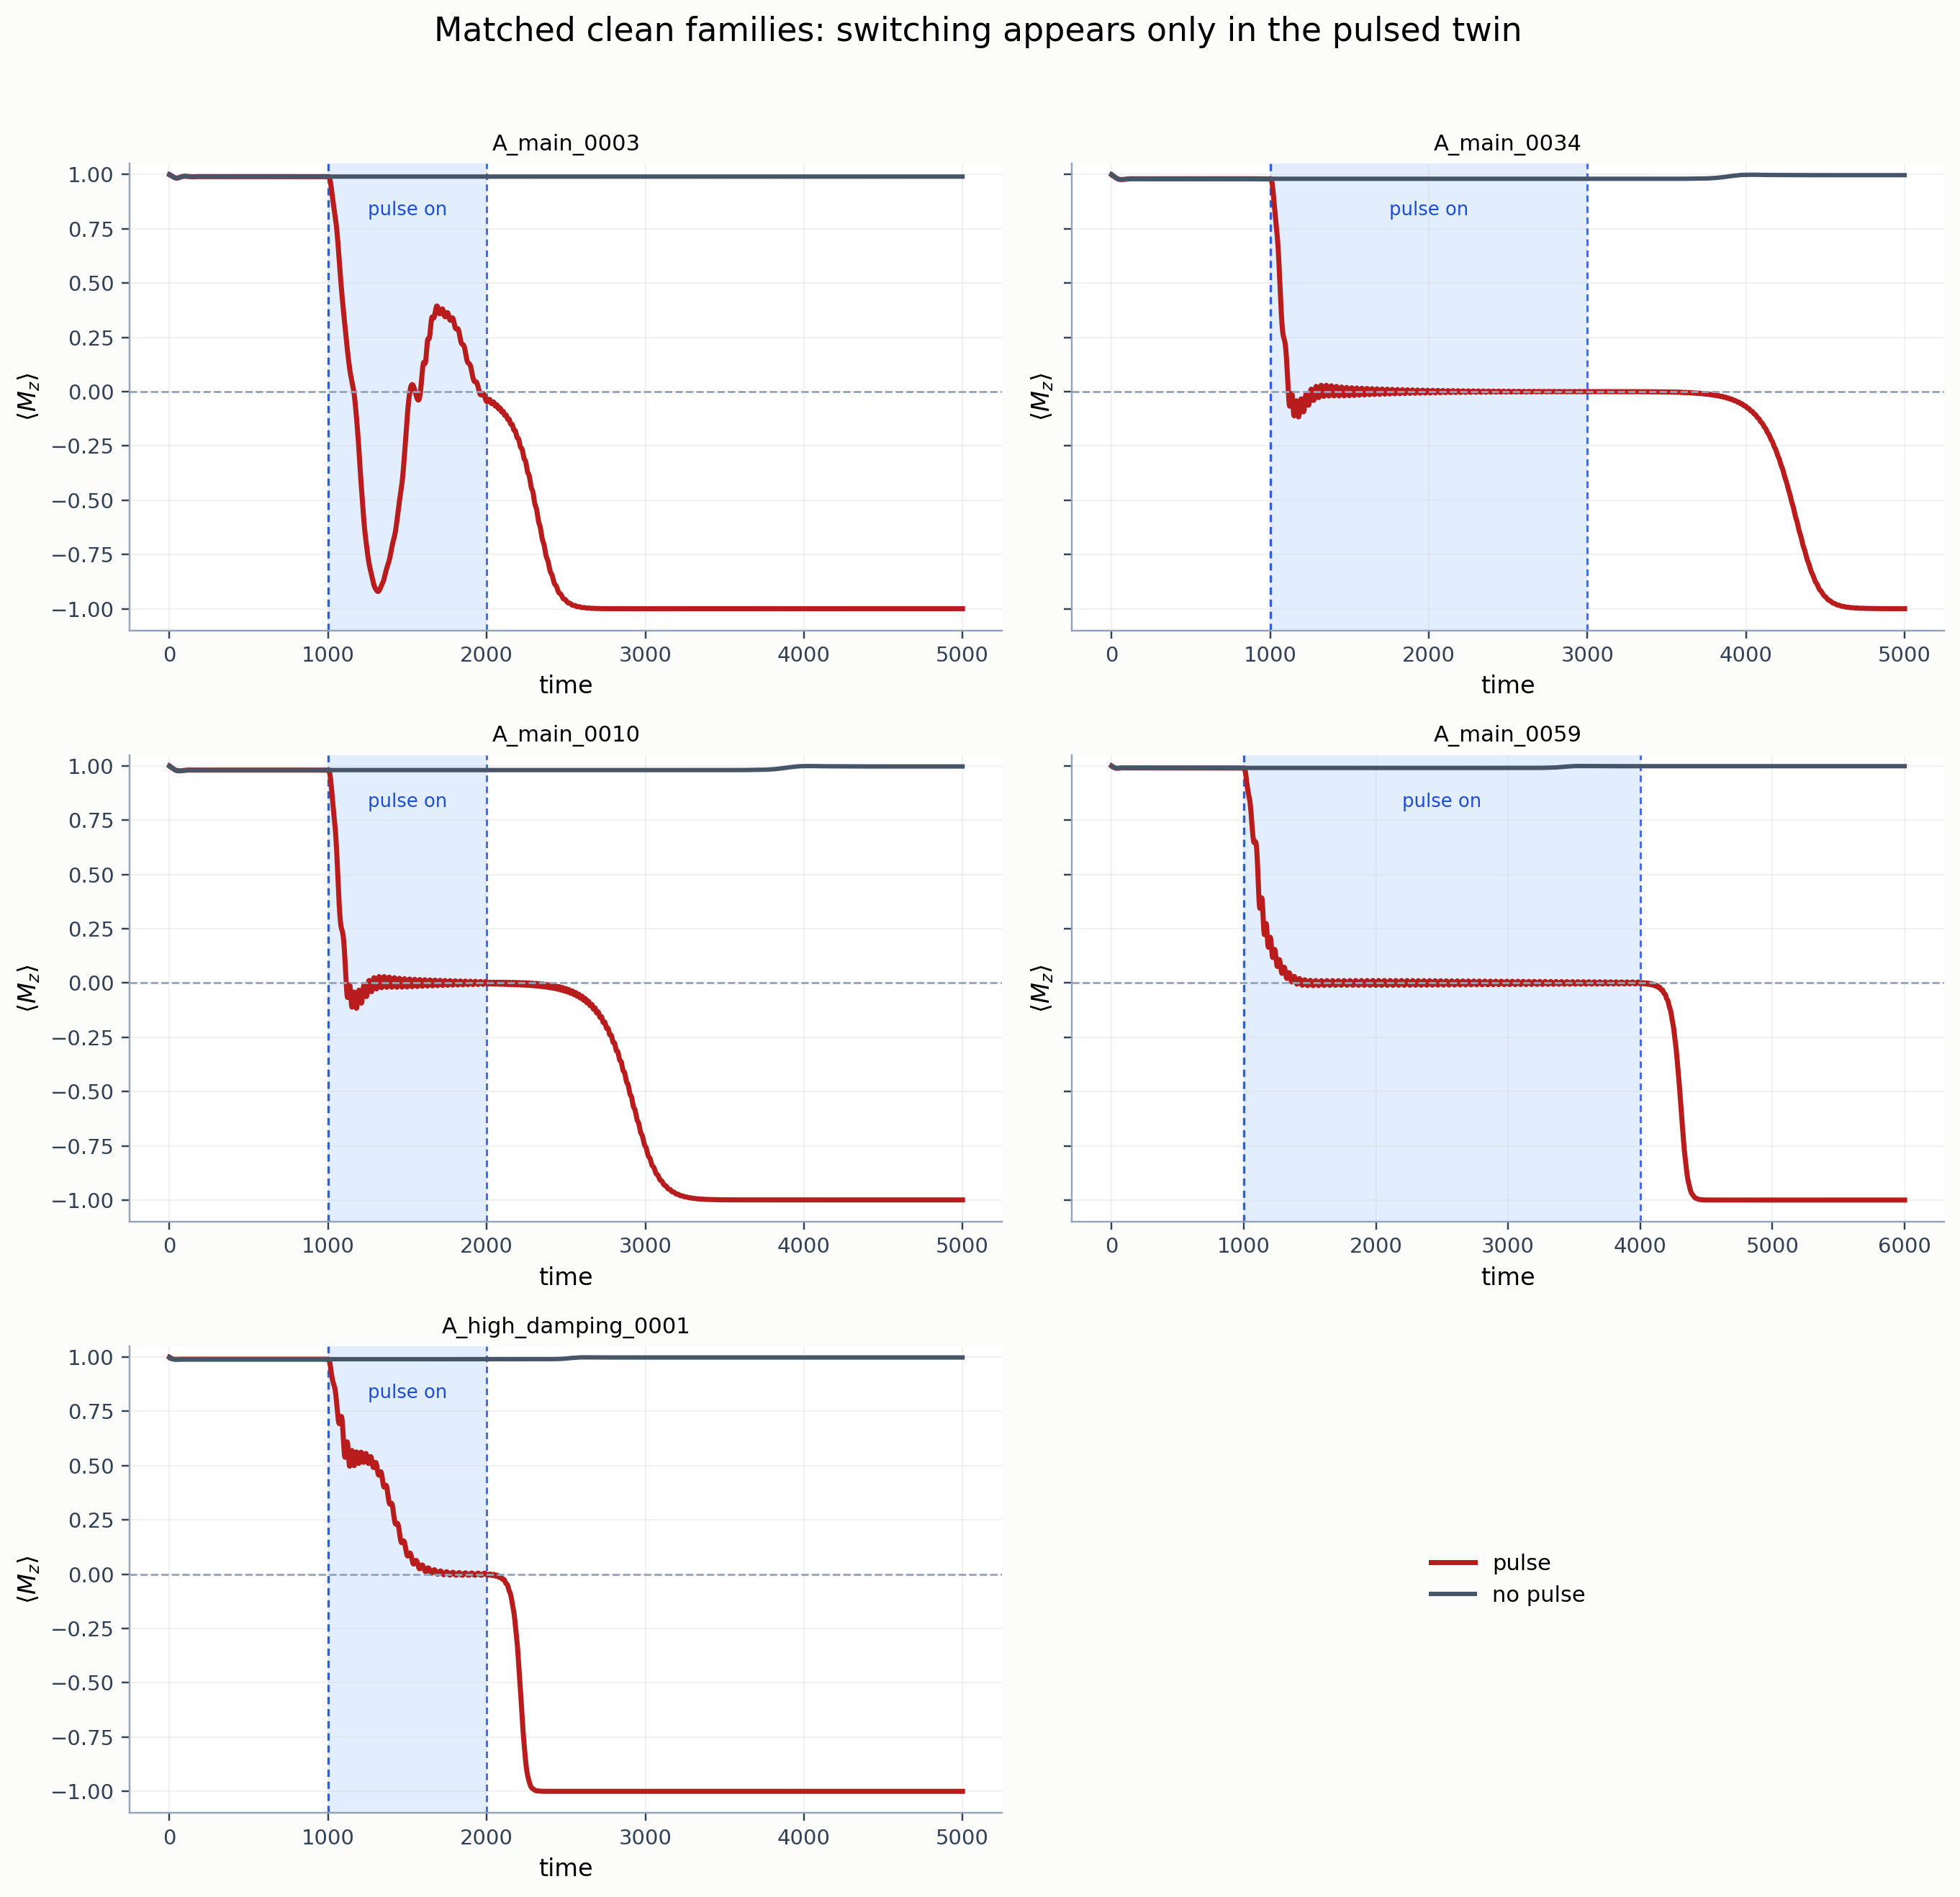
\includegraphics[width=0.95\textwidth]{figures/clean_family_avgMz_grid.png}
  \caption{Matched magnetic dynamics for the five clean families. The pulsed member reverses and remains near \(-1\), while the no-pulse control remains near \(+1\). This is the cleanest direct evidence that the drive, not generic relaxation, is responsible for the switching in these families.}
  \label{fig:clean-avgmz}
\end{figure}

\begin{figure}[H]
  \centering
  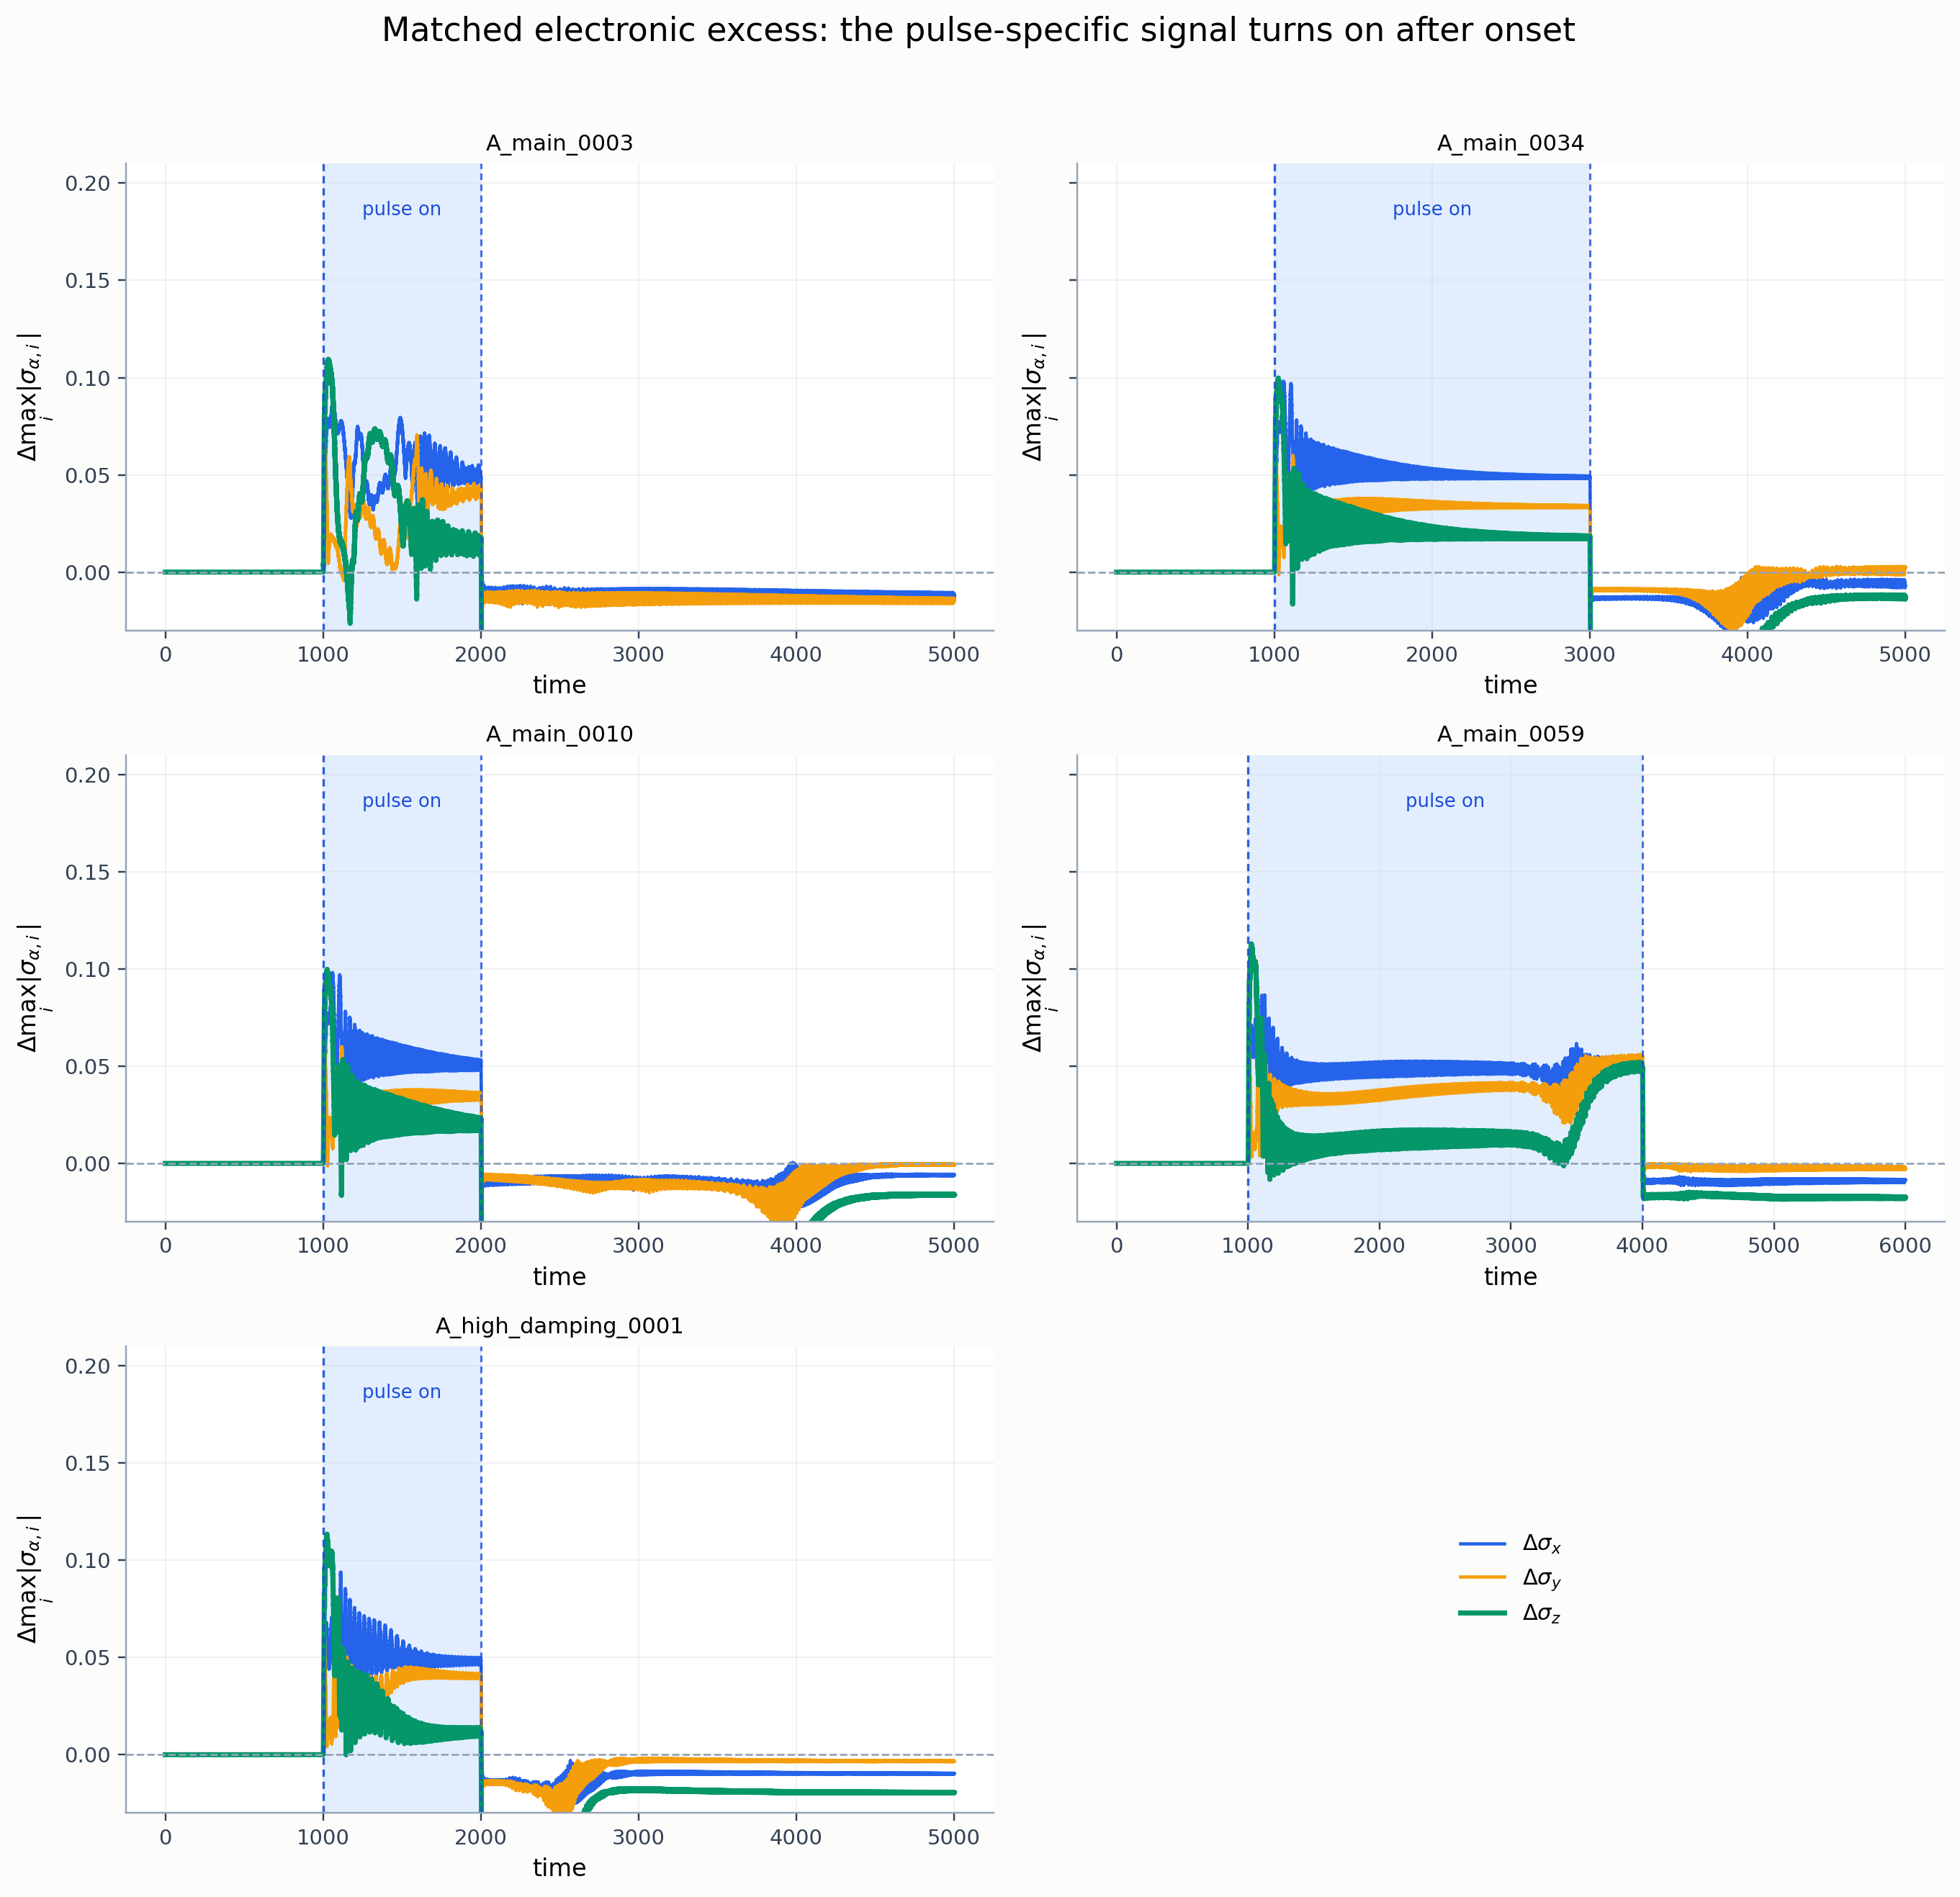
\includegraphics[width=0.95\textwidth]{figures/clean_family_excess_grid.png}
  \caption{Matched pulse-minus-no-pulse electronic excess for the five clean families. The excess is zero before the pulse in the analysis output, appears only after pulse onset, and is consistently dominated by the \(z\) component.}
  \label{fig:clean-excess}
\end{figure}

Table~\ref{tab:phase2-summary} gives the clean-family numbers in a compact form that fits on the page. The strongest case is \texttt{goal6\_A\_main\_0003}, whose excess peak reaches \(0.1893\) at \(t=1327.9\). The other four cases cluster tightly between \(0.1672\) and \(0.1715\), which is strong evidence for a reproducible family-level effect rather than a single isolated outlier.

\begin{table}[H]
\centering
\caption{Compact quantitative summary of the five clean matched pulse/control pairs.}
\label{tab:phase2-summary}
\small
\begin{tabularx}{\textwidth}{>{\raggedright\arraybackslash}p{0.18\textwidth} >{\raggedright\arraybackslash}p{0.17\textwidth} >{\raggedright\arraybackslash}p{0.11\textwidth} >{\raggedright\arraybackslash}p{0.11\textwidth} >{\raggedright\arraybackslash}p{0.11\textwidth} >{\raggedright\arraybackslash}p{0.11\textwidth} Y}
\toprule
Case & Key varying parameters & First strong drop time & Zero-cross time & Peak \(\Delta\sigma\) & Peak time & Final \(\langle M_z\rangle\) pulse / control \\
\midrule
\texttt{0003} & \(j_{ani}=0.03\), damping \(=0.3\), width \(=1000\) & 1026.9 & 1162.0 & 0.1893 (\(z\)) & 1327.9 & -0.9997 / 0.9904 \\
\texttt{0034} & \(j_{ani}=0.01\), damping \(=0.7\), width \(=2000\) & 1021.0 & 1114.0 & 0.1672 (\(z\)) & 1126.0 & -0.9999 / 0.9971 \\
\texttt{0010} & \(j_{ani}=0.01\), damping \(=0.7\), width \(=1000\) & 1021.0 & 1114.0 & 0.1672 (\(z\)) & 1126.0 & -0.9994 / 0.9971 \\
\texttt{0059} & \(j_{ani}=0.03\), damping \(=0.7\), width \(=3000\) & 1027.5 & 1397.2 & 0.1715 (\(z\)) & 1124.0 & -1.0000 / 0.9984 \\
\texttt{A\_hd\_0001} & \(j_{ani}=0.03\), damping \(=1.0\), width \(=1000\) & 1026.3 & 1724.1 & 0.1678 (\(z\)) & 1110.3 & -1.0000 / 0.9984 \\
\bottomrule
\end{tabularx}
\normalsize
\end{table}

\section{Physical conclusions}
The most defensible conclusions of the campaign are now the following.

\begin{enumerate}
\item \textbf{The project has identified a genuine pulse-driven switching regime.} The broad scan shows large pulse-locked destabilization of the initial \(+z\) state, especially at low anisotropy.

\item \textbf{Clean retained switching is established in a restricted but reproducible part of parameter space.} In Branch A/\texttt{hsneq} and in the high-damping strip, matched pulsed runs finish near \(-1\) while their no-pulse twins remain near \(+1\).

\item \textbf{At least two switching pathways are present.} Some trajectories invert strongly during the pulse and retain immediately; others undergo only a modest in-pulse response but then continue collapsing after the pulse into the reversed basin.

\item \textbf{The clean families show a pulse-specific electronic fingerprint.} After matched subtraction, the excess is absent before the pulse, appears only after onset, and is always strongest in the \(z\) channel, the channel aligned with the switching axis.

\item \textbf{Baseline control logic changes the physics, not merely the bookkeeping.} The Branch B/\texttt{hsfull} family cannot yet support a clean switching claim because the no-pulse baseline already exhibits negative excursions and near-zero or slightly negative final states.

\item \textbf{The current result is branch selective, not universal.} The correct statement today is that pulse-driven switching is established for the clean families and still unresolved for Branch B, rather than claimed for every family in the scanned window.
\end{enumerate}

\section{Most important next step}
The most useful next step is not a broader uncontrolled scan. It is a targeted study of why the Branch B/\texttt{hsfull} neighborhood sits so close to a sign-indefinite no-pulse baseline. Resolving that question will determine whether the present mechanism extends beyond the clean Branch A regime or whether the switching physics is intrinsically family selective in this parameter window.

\begin{thebibliography}{9}

\bibitem{gilbert2004}
T. L. Gilbert,
\textit{A phenomenological theory of damping in ferromagnetic materials},
IEEE Transactions on Magnetics \textbf{40}, 3443--3449 (2004).

\bibitem{petrovic2018}
D. Petrovi\'c, P. Plech\'a\v{c}, and B. K. Nikoli\'c,
\textit{Anomalous spin torque generated by nonequilibrium spin density in interacting quantum-classical spin systems},
Physical Review Letters \textbf{121}, 267203 (2018).

\bibitem{petrovic2019}
D. Petrovi\'c, P. Plech\'a\v{c}, and B. K. Nikoli\'c,
\textit{Time-retarded damping and magnetic inertia in the Landau--Lifshitz--Gilbert equation self-consistently coupled to electronic time-dependent nonequilibrium Green functions},
Physical Review B \textbf{99}, 134409 (2019).

\bibitem{manchon2019}
A. Manchon, J. \v{Z}elezn\'y, I. M. Miron, T. Jungwirth, J. Sinova, A. Thiaville, K. Garello, and P. Gambardella,
\textit{Current-induced spin-orbit torques in ferromagnetic and antiferromagnetic systems},
Reviews of Modern Physics \textbf{91}, 035004 (2019).

\end{thebibliography}

\end{document}
